\documentclass[11pt,a4paper]{article}

%======================================================================
% Title, author and date
%======================================================================

\title{
	Projektdokumentation\\
	Transportüberwachungssystem Roadrunner
}
\author{
	Franziskus Domig, B.Sc.\\
		\and
	Stefan Gassner, B.Sc.\\
		\and
	Wolfgang Halbeisen, B.Sc.\\
		\and
	Matthias Schmid, B.Sc.\\	
}
\date{\today}

%======================================================================
% Packages
%======================================================================

%%%%%%%%%%%%%%%%%%%%%%%%%%%%%%%%%%%%%%%%%%%%%%%%%%%%%%%%%%%%%%%%%%%%%
% Packages

% für \hyphenation mit Umlauten
\usepackage[T1]{fontenc}
\usepackage[utf8]{inputenc}
\usepackage[ngerman,english]{babel}

% Times-Roman-Schrift (auch für mathematische Formeln)
\usepackage{mathptmx} 

% comments
\usepackage{verbatim} 

% Zum Setzen von URLs
\usepackage{color}
\usepackage{alltt}
\definecolor{darkred}{rgb}{.25,0,0}
\definecolor{darkgreen}{rgb}{0,.2,0}
\definecolor{darkmagenta}{rgb}{.2,0,.2}
\definecolor{darkcyan}{rgb}{0,.15,.15}

\usepackage[plainpages=false,bookmarks=true,bookmarksopen=true,colorlinks=true,
  linkcolor=darkred,citecolor=darkgreen,filecolor=darkmagenta,
  menucolor=darkred,urlcolor=darkcyan]{hyperref}

% Zeilenabstand
\renewcommand{\baselinestretch}{1.5}

% anhang
\usepackage[toc,page]{appendix}

% pdflatex: Bilder in den Formaten .jpeg, .png und .pdf
% latex: Bilder im .eps-Format
\usepackage{graphicx}

\usepackage{fancyhdr} % Positionierung der Seitenzahlen
\fancyhead{}
\fancyfoot[C]{\Roman{page}}
\renewcommand{\headrulewidth}{0pt}
\setlength{\headheight}{13.6pt} % behebt headheight Warning

 % behebt headheight Warning
\setlength{\headheight}{13.6pt}

% Korrektes Format für Nummerierung von Abbildungen (figure) und
% Tabellen (table): <Kapitelnummer>.<Abbildungsnummer>
\makeatletter
\@addtoreset{figure}{section}
\renewcommand{\thefigure}{\thesection.\arabic{figure}}
\@addtoreset{table}{section}
\renewcommand{\thetable}{\thesection.\arabic{table}}
\makeatother

% Listings für Sourcecode
\usepackage{listings}
  \usepackage{courier}
 \lstset{
        basicstyle=\footnotesize\ttfamily, % Standardschrift
        numbers=left,               % Ort der Zeilennummern
        numberstyle=\tiny,          % Stil der Zeilennummern
        %stepnumber=2,               % Abstand zwischen den Zeilennummern
        numbersep=5pt,              % Abstand der Nummern zum Text
        tabsize=2,                  % Groesse von Tabs
        extendedchars=true,         %
        breaklines=true,            % Zeilen werden Umgebrochen
        keywordstyle=\color{red},
        frame=b,         
        keywordstyle=[1]{\color{DarkSkyBlue}},    % Stil der Keywords
        keywordstyle=[2]{\color{DarkScarletRed}},    %
        keywordstyle=[3]{\bfseries},    %
        keywordstyle=[4]{\color{DarkPlum}},    %
        keywordstyle=[5]{\color{SkyBlue}},    %
		stringstyle={\color{Chocolate}},
        showspaces=false,           % Leerzeichen anzeigen ?
        showtabs=false,             % Tabs anzeigen ?
        xleftmargin=17pt,
        framexleftmargin=17pt,
        framexrightmargin=5pt,
        framexbottommargin=4pt,
        backgroundcolor=\color{Aluminium1},
        showstringspaces=false,      % Leerzeichen in Strings anzeigen ?
		%language=php
		morekeywords=[1]{Interface,return,static,function}
}
    %\DeclareCaptionFont{blue}{\color{blue}} 

  %\captionsetup[lstlisting]{singlelinecheck=false, labelfont={blue}, textfont={blue}}
  \usepackage{caption}
\DeclareCaptionFont{white}{\color{white}}
\DeclareCaptionFormat{listing}{\colorbox[cmyk]{0.43, 0.35, 0.35,0.01}{\parbox{\textwidth}{\hspace{15pt}#1#2#3}}}
\captionsetup[lstlisting]{format=listing,labelfont=white,textfont=white, singlelinecheck=false, margin=0pt, font={bf,footnotesize}}
\renewcommand\lstlistingname{Codeblock}
 

\sloppy % Damit LaTeX nicht so viel über "overfull hbox" u.Ä. meckert

% Ränder
\addtolength{\topmargin}{-16mm}
\setlength{\oddsidemargin}{40mm}
\setlength{\evensidemargin}{40mm}
\addtolength{\oddsidemargin}{-1in}
\addtolength{\evensidemargin}{-1in}
\setlength{\textwidth}{13cm}
\addtolength{\textheight}{34mm}
%______________________________________________________________________

% Verhindert Hurenkinder & Schusterjungen
\clubpenalty = 10000
\widowpenalty = 10000
\displaywidowpenalty = 10000



%======================================================================
% PDF settings
%======================================================================

\hypersetup{
	pdfauthor = {
		Franziskus Domig, B.Sc;
		Stefan Gassner, B.Sc.;
		Wolfgang Halbeisen, BSc;
		Matthias Schmid, B.Sc.
	},
	pdftitle = {Projekt Dokumentation Roadrunner},
	pdfkeywords = {Roadrunner, Dokumentation, Transport, Logistik,
		Transportüberwachung},
}

%======================================================================
%      Document
%======================================================================

\begin{document}

\selectlanguage{ngerman}

\pagestyle{empty} % Vorerst keine Seitenzahlen
\pagenumbering{alpha} % Unsichtbare alphabetische Nummerierung

\begin{center}


\includegraphics[width=60mm]{files/logo-fhv.png}

\vspace{4cm}
{\large\textbf{Projektdokumentation}}\vspace{.5cm}

{\LARGE Transportüberwachungssystem Roadrunner}

\end{center}

\vspace{13cm}


\begin{tabular}{ll}
	Projektteam: & Franziskus Domig, Bsc; Stefan Gassner, BSc;\\
	     	& Wolfgang Halbeisen, BSc; Matthias Schmid, BSc\\
	Bearbeitung: & Dornbirn, im Sommersemester 2011\\
	Betreuer:    & Prof.(FH) DI Wolfgang Auer\\
\end{tabular}

%______________________________________________________________________

\clearpage
\pagestyle{fancy}
\pagenumbering{roman} % Römische Seitenzahlen
\setcounter{page}{1}

\begin{abstract}
	In dieser Arbeit wird die Erstellung eines Transportüberwachungssystems
		für Arzneimittel erläutert. Es werden die Komponenten einer mobilen
		Applikation für die	Android Plattform beschrieben, ein Backendserver
		mit CouchDB erläutert sowie die Überwachung mit einer Webapplikation
		dargestellt. Um das	implementierte System für ein reales Szenario
		verwenden zu können, werden abschließend die wirtschaftlichen Aspekte
		analysiert.
\end{abstract}

% Abstract in english
\begin{otherlanguage}{english}
	\begin{abstract}
		This paper describes the development of a monitoring and tracing system
			for pharmaceutical products. Furthermore the development of a
			mobile application for the Android platform as well as the
			backendserver with a CouchDB database and the corresponding
			webapplication are described in detail. An economical reflection on
			the developed system is given in a concluding section.
	\end{abstract}
\end{otherlanguage}

\clearpage
\tableofcontents

\clearpage
\pagenumbering{arabic}
\setcounter{page}{1}

% Geändertes Format für Seitenränder, arabische Seitenzahlen
\fancyfoot[CO]{\thepage}

\section{Motivation}

In diesem Projekt haben wir uns auf die Entwicklung von Software konzentriert.
	Hardware sowie entsprechende Sensoren werden simuliert. Wir haben uns in
	neuen Technologien, teilweise sogar in Beta-Versionen, eingearbeitet und 
	diese exzessiv in diesem Projekt verwendet.

Als Softwareentwicklungsprozess wurde \emph{Test-Driven-Development} gewählt.
	Hierzu wurden nahezu alle entwickelten Komponenten mit \emph{Unit-Tests}
	getestet sowie wenn möglich auf einem \emph{Continius-Integration}-Server
	bei jeder Änderung automatisiert getestet.
	
TODO: mehr Inhalt

\clearpage
\section{Projektanforderungen}
\label{sec:requirements}

Das Ziel dieses Projekts ist es, ein System zur lückenlosen Transportüberwachung
	zu entwickeln. Hierzu sollen Produkt, welche erst im Rahmen des Projekts zu
	spezifizieren sind, überwacht werden. Es soll nach einem Transport möglich
	sein, eindeutig nachvollziehen zu können, welche Sensor-Daten zu jedem
	Zeitpunkt aufgezeichnet wurde.
	
TODO: mehr Inhalt

\clearpage
\section{Technologie}
\label{sec:technology}

In diesem Abschnitt werden die von diesem Projekt verwendeten Technologien erläutert. Insbesondere werden die Gründe beschrieben, weswegen diese Technologien eingesetzt und anderen vorgezogen werden. Die Vor- sowie Nachteile der entsprechenden Technologien werden gegenübergestellt und besprochen. Zugleich werden die entsprechenden Technologien auf ihre Tauglichkeit in einem real logistischen Szenario geprüft.

\subsection{CouchDB}
\label{subsec:couchdb}
CouchDB\footnote{The Apache CouchDB Project, \url{http://couchdb.apache.org/}} ist eine auf die Verwaltung von Dokumenten basierte Datenbank. CouchDB kann ähnlich wie das MapReduce Framework von Google\footnote{vgl. \url{http://en.wikipedia.org/wiki/MapReduce}} abgefragt sowie indiziert werden.

TODO: Ausführlicher beschreiben.

\subsection{Node.js}
\label{subsec:nodejs}

Node.js ist ein ereignisgesteuertes I/O Framework für die V8 JavaScript Engine \cite{Wikipedia10a}. Diese wurde in C++ sowie JavaScript entwickelt und liegt in einer MIT-Lizenz vor, welches es für dieses Projekt einsetzbar macht und zugleich auch in einem realen Szenario eingesetzt werden könnte.

Mit Node.js können mit wenigen Zeilen Code, Server-Applikationen programmiert werden. Es wird hierzu auf einem Interface (IP) sowie einem beliebigen Port eine JavaScript Callback-Funktion registriert, welche bei einem Zugriff aufgerufen wird. Dies macht es sehr einfach, Sensoren in diesem System zu simulieren, welche via HTTP-Requests ``ausgelesen'' werden können.


\subsection{PHP - Silex}

PHP ist eine dynamische Skriptsprache, die speziell für den Einsatz auf Webservern entwickelt wurde. Jegliche Anfrage an eine PHP-Datei auf einem entsprechend konfigurierten Webserver wird durch die \emph{PHP-Runtime} interpretiert. Dabei wird eine passende Antwort generiert und durch den Webserver an den Client gesendet. Dies stellt die Basis für eine dynamische Webseite mit PHP dar. PHP ist verfügbar für eine breite Anzahl an Webservern, sowie für unterschiedlichste Plattformen wie Linux, Mac OS X, Windows oder Unix.

Silex\footnote{vgl. \url{http://silex-project.org}} ist ein Mikroframework für PHP 5.3. Es basiert wiederum auf dem Kern des Symfony2\footnote{vgl. \url{http://symfony.com}} Framework.

\subsection{Android/Java}

TODO

\subsection{Barscanner}

TODO

\clearpage
\section{Datenbank}

Bei einem Überwachungssystem für Warentransporte werden sehr viele Daten entstehen. Diese Daten gilt es zu Verwalten und deren Integrität sicherzustellen. In diesem Kapitel werden unterschiedliche Möglichkeiten der Datenverwaltung betrachtet und erläutert welches System für das Projekt Roadrunner verwendet wird.

\subsection{Datenbankinstanzen}

Anfallende Daten müssen persistent gespeichert werden. Diese Speicherung wird in eine Datenbank durchgeführt. Genauer betrachtet werden die Daten in einer Instanz einer Datenbank gespeichert. Es gilt zu unterscheiden ob eine Instanz einer Datenbank verwendet wird oder mehrere Instanzen verwendet werden und diese synchron gehalten werden.

\begin{description}
	\item[Eine Instanz] Bei der Verwendung einer Datenbankinstanz gibt es einen zentralen Datenbankserver. Alle Daten werden von dieser Instanz gelesen und geschrieben. Der Vorteil dabei ist, dass alle gespeicherten Daten auf dieser Instanz sofort zur Verfügung stehen. Der Nachteil ist, dass die Datenbank für alle Clients durchgehend zur Verfügung stehen muss.
	\item[Mehrere Instanzen - Jeder synchronisiert mit jedem] Wenn mehrere Instanzen einer Datenbank verwendet werden gilt es diese synchron zu halten. Dies bedeutet, wenn auf einer Instanz Daten erzeugt werden, müssen diese mit anderen Instanzen synchronisiert werden. Eine Möglichkeit ist, dass jede Instanz mit allen anderen Instanzen synchronisiert wird. Dies wäre eine Lösung, wenn es eine definierte Menge von Instanzen gibt und jede Instanz von jeder Instanz aus erreicht werden kann. Dadurch ergibt sich Fehlertoleranz gegenüber Ausfällen von einzelnen Datenbankinstanzen, da die Daten auf jeder Instanz vorliegen und es keine zentrale Masterinstanz gibt.
	\item [Mehrere Instanzen - Jeder synchronisiert mit der Masterinstanz] Anstatt dass jede Instanz mit jeder anderen Instanz synchronisiert wird kann auch eine zentrale Masterinstanz verwendet werden. Diese zentrale Instanz hält alle Daten und verteilt diese Daten wenn nötig auf andere Instanzen. Diese bedeutet wenn eine Clientinstanz neue Daten generiert hat werden diese zur Masterinstanz gesendet und wenn der Client bestimmte Daten benötigt kann er diese bei der Masterinstanz abholen. Dadurch ergibt sich aber ein zentraler Fehlerpunkt. Wenn die Masterinstanz ausfällt ist keine Datenverteilung mehr möglich. 
\end{description}

Da beim Roadrunner-Projekt die Daten auf mobilen Geräten erzeugt werden und diese oft auch offline arbeiten, müssen die Daten auf dem Gerät ebenfalls gespeichert werden. Diese Daten werden auf dem Gerät in einer Datenbankinstanz gespeichert. Da es einem mobilen Gerät nicht möglich ist zu allen anderen mobilen Geräten im System Kontakt aufzunehmen wird eine zentrale Masterinstanz verwendet. Auf ein mobiles Gerät werden nur solche Daten gespeichert, die für die Abwicklung der Lieferaufträge benötigt werden.

\subsection{Datenspeicherung}

Daten können in einer Datenbank auf unterschiedliche Arten gespeichert werden. Dieser Abschnitt beschreibt die unterschiedlichen Speicherungsarten und beschreibt ob diese für das Projekt Roadrunner verwendet werden können.

\begin{description}
	\item[Relationale Datenbank] In einer relationalen Datenbank werden Daten in einer Tabelle gespeichert. Tabellen werden über PrimaryKey-ForeignKey-Verknüpfungen miteinander in Verbindung gebracht. Ein Eintrag in eine Tabelle, die auf eine andere Tabelle verweist, kann nur durchgeführt werden wenn der Eintrag auf den verweisen wird in der anderen Tabelle existiert. Somit müssten sehr viele Daten auf die mobilen Geräte verteilt werden. Ein Beispiel: Ein Temperatur-Log-Eintrag gehört zu einem Sensor und zu einem Warengut. Das Warengut befindet sich in einem Transportbehälter und muss somit mit diesem Verknüpft werden. Der Transportbehälter hat ein Fahrzeug. Ein Fahrzeug gehört zu einem Fuhrpark usw. Die Verwendung einer relationalen Datenbank auf einem mobilen Gerät wäre nur möglich wenn unterschiedliche Datenbankschemas für die Instanzen der mobilen Geräte und des Masters verwendet werden. 
	\item[Objektorientierte Datenbank] Die Daten werden direkt als Objekte in die Datenbank gespeichert. Da auf den mobilen Geräten aber Java-Objekte bestehen und auf der Webapplikation PHP-Objekte verwendet werden ist diese Lösung nicht ohne intensiven Programmieraufwand für die Konvertierung möglich.
	\item[Dokumentdatenbank] Die Daten werden als Dokumente in die Datenbank gespeichert. Ein Log-Eintrag ist ein Beispiel solch eines Dokumentes. Dokumente sind für sich unabhängige Datensätze die beliebig in einem System verteilt werden können. Dokumente haben Versionsnummern. Anhand der Versionsnummer erkennt eine Datenbankinstanz ob es eine alte Version eines Dokumentes besitzt und kann bei der Masterinstanz eine neue Version des Dokumentes abholen.
\end{description}

Bei Roadrunner wird eine verteilte Dokumentdatenbank verwendet. Die verwendete Datenbank verwendet als Dokumentstruktur JSON. Für JSON gibt es eine hohe Integration in Java und PHP und ist somit eine einfach zu verwendende Datenstruktur.

\subsection{Datenverteilung}

Daten können auf unterschiedliche Arten im System verteilt werden. Eine Möglichkeit wäre die Daten aus der mobilen Datenbankinstanz in die Applikation zu lesen und das Senden der Daten an die Masterinstanz über die Applikation durchzuführen. Eine andere Möglichkeit ist es, die Datenbanksynchronisierung direkt von den Datenbanken durchführen zu lassen. 

Bei der verwendeten Datenbank im Roadrunner-Projekt wird die Synchronisierung der Daten von den Datenbankinstanzen durchgeführt. Diese Synchronisierung nennt sich Replizierung und es kann dabei angegeben werden welche Daten synchronisiert werden sollen.

\subsection{CouchDB}

Dieser Abschnitt beschreibt wie CouchDB die Anforderungen erfüllt.

\subsection{Alternative Datenbanksysteme}

Dieser Abschnitt beschreibt die möglichen alternativen Datenbanksysteme (z.B. Cassandra) und warum CouchDB als Datenbanksystem ausgewählt wurde.


\clearpage
\section{CouchDB}

\subsection{Dokumentstruktur}

\subsection{Designdokumente}

\subsection{Replizierung}

\subsection{MapReduce}

MapReduce ist ein Framework von Google, dass entwickelt wurde damit sehr große Datenmengen parallell bearbeitet werden können. CouchDB verwendet ebenfalls einen MapReduce-Anstaz um Daten aus der Datenbank zu lesen. Anhand eines Beispieles wird die Funktionsweise von MapReduce vorgestellt.

Das Beispiel beantwortet folgende Problemstellung: Welche Waren wurden gescannt und somit als geladen gekennzeichnet?

\subsubsection{Map - Phase}

Auf jedes Document in der Datenbank wird die Map-Methode angewendet. In einer Map-Methode werden Key-Value-Paarungen gebildet. Jedes Document in der Datenbank kann eine beliebige Anzahl an Key-Value-Paarungen generieren. Diese Key-Value-Paarungen werden in einem B-Tree gespeichert. Ändert sich nun ein Dokument müssen nur die entsprechenden Paarungen in dem B-Tree angepasst werden. 

\subsubsection{Reduce - Phase}

In der Reduce-Phase wird auf jeden Node in dem Tree die Reduce-Methode angewendet. Ziel der Reduce-Methode ist es die Datenmenge zu minimieren. Auf jede Node kann die Reduce-Methode beliebig oft angewendet werden. Daher wird die Reduce und die Rereduce-Phase unterschieden.

\subsection{CouchDB auf Android}

\subsection{CouchApp}



\clearpage
\section{Android Applikation}
\label{sec:android}

Als Hauptsystem in diesem Projekt wurde eine Applikation für die Android
	Plattform erstellt. Diese Applikation dient der mobilen Überwachung
	von Lieferungen bzw. den Gegenständen einer Lieferung.

TODO: Was ist Android? Was sind Vor- und Nachteile? Was kann man damit alles
	erreichen? Wo sind die Grenzen?
	
\subsection{Benutzung}

TODO	

\subsection{Implementierung}

TODO

\subsection{Mögliche Erweiterungen}

TODO

\subsection{Verwendung in einem realen System}

TODO

\clearpage
\section{GIT}

\subsection{Unterschiede zu SVN}

\subsection{Arbeitsweise mit GIT}

\subsection{Mögliche Probleme}



\clearpage
\section{Usecases}


\begin{itemize}
  \item Wareneingang
  	\subitem registriert Pakete im System
  	\subitem klebt QR-Code auf Pakete

	\item Logister plant und erstellt Lieferungen (neue Auftragsnummer wird
	generiert) \subitem wählt Pakete aus (können mit Sensoren bestückt sein)
		\subitem wählt Fahrer aus 
		\subitem wählt Transportmittel (können mit Sensoren bestückt sein) für
		Lieferungen aus
		\subitem trägt Zielort und Auftraggeber ein
  	
  \item Transporteur
  	\subitem holt oder hat Device mit Roadrunner App
  	\subitem loggt sich im Roadrunner System ein
  		\subsubitem mit Benutzerdaten wird sein/e aktuelle/r Auftrag/Lieferung aufs
  		Device synchronisiert ODER 
  		\subsubitem scannt Pakete und lädt sie in das vom Logistiker ausgwählte
  		Transportmittel
\end{itemize}

\paragraph{Daten-Synchronisierung}
	\textbf{Vorbedingungen: }
	\begin{itemize}
	  \item Transporteur hat sich in der System-App eingeloggt
	\end{itemize}
	
	Die Daten-Synchronisierung oder Replizierung wird durch das Einloggen im
	System angestoßen. Das mobile Gerät erhält folgende Information:
	\begin{itemize}
	  \item Adressen der Sensoren, die das Gerät überwachen sollte
	  \item alle Produkte, Pakete der aktuellen Lieferung, sowie Zielort, etc.
	  \item Überwachungs-Thresholds der Pakete
	\end{itemize}
\par


\clearpage
\section{Iteration 1}

\subsection{Ziele}

\begin{itemize}
  \item Produkte können erzeugt werden.
  \item Produkte können eingelagert werden.
  \item Produkte können ausgelagert werden.
\end{itemize}

\subsection{UML}

\begin{figure}
	\centering
		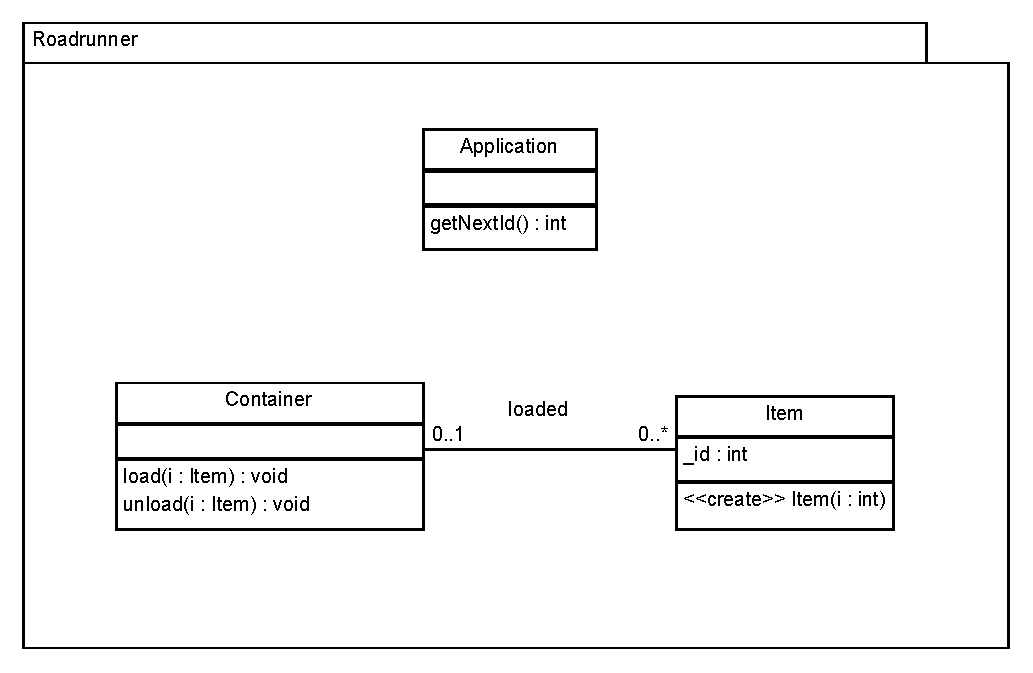
\includegraphics[width=\textwidth]{files/pdf/Iteration1.pdf}
	\caption{Iteration 1}
	\label{fig:Iteration1}
\end{figure}


\clearpage
\section{Sicherheit}

\subsection{Zeitsynchronisierung}

In diesem Abschnitt werden Probleme besprochen, die durch fehlerhafte respektive
mangelhaft durchdachte Zeitsynchronisierung oder Verbindungsabbruch entstehen
können.


\paragraph{Problem durch falsche Zeitstempel bei Logeinträgen:}
Betrachtet wird das Szenario ``Umladevorgang eines Produktes''. Das mobile
Gerät der Transporteinheit wird benutzt um den Ausladevorgang aus einem
Container im System zu verarbeiten. Mit dem scannen des Produkts wird auf dem
mobilen Gerät der Transporteinheit ein Logeintrag in dessen lokale Datenbank
erstellt. Genauso wird beim darauffolgenden Ladevorgang der Umladestation ein
Logeintrag auf dessen Gerät erstellt. Wenn das System mit absoluter Zeit
arbeitet und die Uhrzeit des Geräts der Transporteinheit vor jener der
Umladestation ist, dann würde im System der Übernahmevorgang der Umladestation
vor dem Ausladevorgang der Transporteinheit stattfinden.
\par
\paragraph{Lösungsansatz:}
Um dieses Problem zu lösen muss relative Zeit eingeführt und synchronisiert
werden. Für die Zeitsynchronisierung können bekannte Algorithmen für verteilte
Systeme eingeführt werden. Mögliche Algorithmen sind
\par

\paragraph{TODO:}
UPV distributed Clocks .. algorithmen herausfinden und oben einfügen\\ 

	Christian's Algorithm, Berkley Algorithm, 
	$http://en.wikipedia.org/wiki/Clock_synchronization$
\par

Grundsätzlich müssen diese Probleme berücksichtigt werden. In unserem
Projekt werden die erwähnten Lösungen aus zeitlichen Gründen und anderer
Zielsetzung nicht implementiert.


\clearpage
\section{Transportüberwachung mittels Sensoren}\label{sensors}
\label{sec:sensors}

In diesem Projekt wurden die Transportüberwachung mittels Sensoren, welche
	von der Android Applikation (siehe Kapitel~\ref{sec:android})) überwacht
	werden, realisiert.
	
Für die in diesem Projekt spezifizierten Anforderungen (siehe Kapitel~\ref{sec:requirements})
	wurde die Temperatur sowie die aktuelle Position eines Gegenstands überwacht. Hierzu
	werden zwei unterschiedliche Sensortypen, welche in den beiden nachfolgenden Abschnitten
	erläutert werden, verwendet. Zusätzlich wurde die Zeitsynchronisation der mobilen Geräte
	mittels eigens entwickelter Synchronisierung (wie in Abschnitt~\ref{subsec:timesync}
	erläutert) realisiert.

\subsection{Temperaturüberwachung}

Temperatursensoren werden in diesem Projekt simuliert. Alle benötigten
	Temperatursensoren werden mit \emph{nodejs}, wie in
	Abschnitt~\ref{subsec:nodejs} erläutert, simuliert.

\subsection{Positionsüberwachung}


%______________________________________________________________________

\cleardoublepage
\begin{thebibliography}{99}
\addcontentsline{toc}{section}{Literaturverzeichnis}

\bibitem[Beck 98]{Beck98}
	K.\ Beck, W.\ Cunningham, R.\ Jeffries:
	Chrysler Goes To ``Extremes'',
	Distributed Systems: Case Study, S. 25-28 October 1998,
	online abrufbar: \url{http://www.xprogramming.com/publications/dc9810cs.pdf}.

\bibitem[Brown 98]{Brown98}
  W.\ H.\ Brown, R.\ C.\ Malveau, H.\ W.\ McCormick III, et al.:
    Anti Patterns Refactoring Software, Architectures, and Projects in Crisis.
    New York: John Wiley \& Sons, Inc., 1998.

\bibitem[Christian 89]{Christian89}
	F.\ Cristian:
	Probabilistic clock synchronization,
	Distributed Computing (Springer) 3 (3), 1998.

\bibitem[Gamma 94]{Gamma94}
  E.\ Gamma, R.\ Helm, R.\ Johnson, J.\ Vlissides:
    Design Patterns: Elements of Reusable Object-Oriented Software,
	MA: Addison-Wesley, 1994.
	
\bibitem[Ottmann 96]{Ottmann96}
  T.\ Ottmann, P.\ Widmayer:
	Algorithmen und Datenstrukturen-3,
	Heidelberg; Berlin; Oxford: Spektrum, Akad. Verlag 1996.

\bibitem[Schmidt 09]{Schmidt09}
  S. \ Schmidt:
	PHP Design Patterns: Entwurfsmuster für die Praxis.,
	Köln: O'Reilly Verlag, 2. Auflage 2009.

%    Web-References
%______________________________________________________________________

\hspace{-\leftmargin}{\Large\bfseries Web-Referenzen} % Wüster Hack %-|

\bibitem[ARGE Pharmazeutika 07]{PHARMIG07}
	Arbeitsgemeinschaft des pharmazeutischen Großhandels Österreichs:
	Codex für den Transport von Arzneimitteln in Österreich
	\url{http://www.argepgh.at/kwpc_Downloads/Pharmarecht%20%D6sterreich/Codex%20Transport%201007.pdf},
	besucht am 15.03.2011.

\bibitem[CouchDB 11]{CouchDB11}
	Apache CouchDB:
	Technical Overview
	\url{http://couchdb.apache.org/docs/overview.html},
	besucht am 22.06.2011.

\bibitem[Fowler 10]{Fowler10}
	M.\ Fowler:
	Richardson Maturity Model: Steps towards the glory of REST
	\url{http://martinfowler.com/articles/richardsonMaturityModel.html},
	besucht am 20.06.2011.
	
\bibitem[Internet Engineering Task Force 11]{IETF11}
	Internet Engineering Task Force:
	A JSON Media Type for Describing the Structure and Meaning of JSON Documents
	\url{http://tools.ietf.org/html/draft-zyp-json-schema-03},
	besucht am 11.05.2011.

\bibitem[Murphy 09]{Murphy09}
	E.\ Murphy:
	CouchDB in Ubuntu
	\url{http://mail-archives.apache.org/mod_mbox/couchdb-dev/200910.mbox/%3C4AD53996.3090104@canonical.com%3E}, besucht am 16.06.2011.

\bibitem[Open Handset Alliance 07]{OHA07}
  Open Handset Alliance
    \url{http://www.openhandsetalliance.com/press_110507.html}, besucht am 23.06.2011.

\bibitem[Torvalds 07]{Torvalds07}
	Linus Torvalds (2005-04-07).
	``Re: Kernel SCM saga..''.
	The linux-kernel mailing list. ``So I'm writing some scripts to try to track
	things a whole lot faster.''
	\url{http://marc.info/?l=linux-kernel&m=111288700902396}, besucht am 18.06.2011.

\bibitem[W3C 11]{W3C11}
	W3C Working Draft 7 April 2011:
	Grid Layout
	\url{http://www.w3.org/TR/css3-grid-layout/}, besucht am 22.06.2011.

\bibitem[Wikipedia 10a]{Wikipedia10a}
  Wikipedia: Node.js
    \url{http://de.wikipedia.org/wiki/Node.js}, besucht am 20.04.2011.
	
\end{thebibliography}


% ende des hauptteils
\fancyhead[R]{} % Keine Kopfzeile mehr oben auf jeder Seite

\end{document}
